\documentclass{ctexart}
\usepackage{minted}
\usepackage{xcolor}
\usepackage{graphicx}


\begin{document}
\title{计算机组成原理 作业2}

\date{\today}
\maketitle
\section*{1}
\subsection*{实验环境}
实验环境为 Arch Linux x86\_64,安装交叉编译工具链的命令如下:

\begin{minted}[frame=lines, linenos, bgcolor=gray!10, tabsize=4]{bash}
sudo pacman -S clang llvm
sudo pacman -S riscv64-unknown-elf-gcc riscv64-unknown-elf-binutils
\end{minted}


安装完后查看版本并验证支持RISCV

\begin{minted}[frame=lines, linenos, bgcolor=gray!10]{bash}
clang --version
clang --print-targets | grep riscv
\end{minted}

\begin{figure}[H]
    \centering
    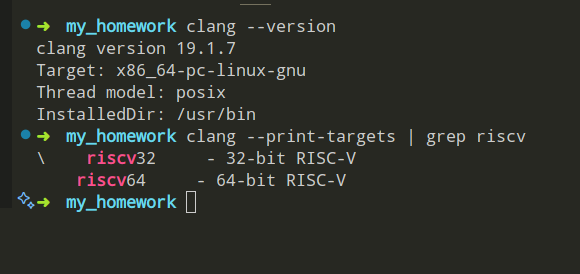
\includegraphics[width=0.8\textwidth]{image.png} % 替换为图片路径
    \caption{安装版本和支持}
    \label{fig:安装版本和支持} 
\end{figure}

安装成功
\subsection*{构建工程}
构建 \texttt{code} 工程,结构如下:
\begin{verbatim}
code
├── src
│   ├── main.c       # 程序的入口点,包含主函数。
│   ├── main.s       # 从 main.c 生成的汇编代码。
│   ├── main2.s      # 从二进制文件反汇编的代码。
│   ├── main.bin     # 为 RISC-V 编译的二进制文件。
├── Makefile         # 用于将项目编译为 32 位 RISC-V 汇编的构建规则。
\end{verbatim}

\begin{itemize}
    \item \texttt{main.s}:从 \texttt{main.c} 生成的汇编代码。
    \item \texttt{main.bin}:为 RISC-V 架构编译的二进制文件。
    \item \texttt{main2.s}:从二进制文件反汇编的代码。
\end{itemize}


在 \texttt{src} 文件夹下创建 \texttt{main.c} 文件,写入以下代码:
\begin{minted}[frame=lines, linenos, bgcolor=gray!10]{c}
int main() {
    char string[8] = {'3', 'b', 'a', '?', '#', '@', '<', '8'};
    for (int i = 0; i < 8; i++) {
        char temp = '\0';
        for (int j = 0; j < 7 - i; j++) {
            if (string[j] <= string[j + 1]) {
                break;
            } else {
                temp = string[j];
                string[j] = string[j + 1];
                string[j + 1] = temp;
            }
        }
    }
    return 0;
}
\end{minted}

根据要求,写出Makefile文件
\begin{minted}[frame=lines, linenos, bgcolor=gray!10]{makefile}
CC=clang
AS=llvm-mc
OBJDUMP=llvm-objdump
CFLAGS=-S -target riscv32 -march=rv32i -mabi=ilp32 -O0 -g3
SRC=src/main.c
ASM=$(SRC:.c=.s)
BIN=$(SRC:.c=.bin)
DISASM=$(SRC:.c=2.s)

.PHONY: all clean

all: $(ASM) $(BIN) $(DISASM)

$(ASM): $(SRC)
    $(CC) $(CFLAGS) -o $@ $<

$(BIN): $(ASM)
    $(AS) -triple=riscv32 -filetype=obj -o $(BIN) $<

$(DISASM): $(BIN)
    $(OBJDUMP) -d --source $(BIN) > $(DISASM)

clean:
    rm -f $(ASM) $(BIN) $(DISASM)
\end{minted}

生成的main2.s有汇编和16进制机器码、源代码关系
\begin{verbatim}

src/main.bin:	file format elf32-littleriscv

Disassembly of section .text:

00000000 <main>:
; int main() {
       0: fe010113     	addi	sp, sp, -0x20
       4: 00112e23     	sw	ra, 0x1c(sp)
       8: 00812c23     	sw	s0, 0x18(sp)
       c: 02010413     	addi	s0, sp, 0x20
      10: 00000513     	li	a0, 0x0
      14: fea42a23     	sw	a0, -0xc(s0)
      18: 383c45b7     	lui	a1, 0x383c4
      1c: 02358593     	addi	a1, a1, 0x23
;     char string[8] = {'3', 'b', 'a', '?', '#', '@', '<', '8'};
      20: feb42823     	sw	a1, -0x10(s0)
      24: 3f6165b7     	lui	a1, 0x3f616
      28: 23358593     	addi	a1, a1, 0x233
      2c: feb42623     	sw	a1, -0x14(s0)

00000030 <.Ltmp1>:
;     for(int i = 0; i < 8; i++)
      30: fea42423     	sw	a0, -0x18(s0)
      34: 0040006f     	j	0x38 <.Ltmp1+0x8>
      38: fe842583     	lw	a1, -0x18(s0)
      3c: 00700513     	li	a0, 0x7
      40: 0ab54863     	blt	a0, a1, 0xf0 <.Ltmp16>
      44: 0040006f     	j	0x48 <.Ltmp1+0x18>
      48: 00000513     	li	a0, 0x0

0000004c <.Ltmp4>:
;         char temp = '\0';
      4c: fea403a3     	sb	a0, -0x19(s0)

00000050 <.Ltmp5>:
;         for(int j = 0; j < 7 - i; j++)
      50: fea42023     	sw	a0, -0x20(s0)
      54: 0040006f     	j	0x58 <.Ltmp5+0x8>
      58: fe042503     	lw	a0, -0x20(s0)
      5c: fe842603     	lw	a2, -0x18(s0)
      60: 00700593     	li	a1, 0x7
      64: 40c585b3     	sub	a1, a1, a2
      68: 06b55a63     	bge	a0, a1, 0xdc <.Ltmp14>
      6c: 0040006f     	j	0x70 <.Ltmp5+0x20>
;             if(string[j] <= string[j + 1])
      70: fe042583     	lw	a1, -0x20(s0)
      74: fec40513     	addi	a0, s0, -0x14
      78: 00b50533     	add	a0, a0, a1
      7c: 00054583     	lbu	a1, 0x0(a0)
      80: 00154503     	lbu	a0, 0x1(a0)
      84: 00b54663     	blt	a0, a1, 0x90 <.Ltmp5+0x40>
      88: 0040006f     	j	0x8c <.Ltmp5+0x3c>
;                 break;
      8c: 0500006f     	j	0xdc <.Ltmp14>
;                 temp = string[j];
      90: fe042503     	lw	a0, -0x20(s0)
      94: fec40613     	addi	a2, s0, -0x14
      98: 00a60533     	add	a0, a2, a0
      9c: 00054503     	lbu	a0, 0x0(a0)
      a0: fea403a3     	sb	a0, -0x19(s0)
;                 string[j] = string[j + 1];
      a4: fe042503     	lw	a0, -0x20(s0)
      a8: 00a605b3     	add	a1, a2, a0
      ac: 0015c503     	lbu	a0, 0x1(a1)
      b0: 00a58023     	sb	a0, 0x0(a1)
;                 string[j + 1] = temp;
      b4: fe744503     	lbu	a0, -0x19(s0)
      b8: fe042583     	lw	a1, -0x20(s0)
      bc: 00c585b3     	add	a1, a1, a2
      c0: 00a580a3     	sb	a0, 0x1(a1)
      c4: 0040006f     	j	0xc8 <.Ltmp5+0x78>
;         }
      c8: 0040006f     	j	0xcc <.Ltmp5+0x7c>
;         for(int j = 0; j < 7 - i; j++)
      cc: fe042503     	lw	a0, -0x20(s0)
      d0: 00150513     	addi	a0, a0, 0x1
      d4: fea42023     	sw	a0, -0x20(s0)
      d8: f81ff06f     	j	0x58 <.Ltmp5+0x8>

000000dc <.Ltmp14>:
;     }
      dc: 0040006f     	j	0xe0 <.Ltmp15>

000000e0 <.Ltmp15>:
;     for(int i = 0; i < 8; i++)
      e0: fe842503     	lw	a0, -0x18(s0)
      e4: 00150513     	addi	a0, a0, 0x1
      e8: fea42423     	sw	a0, -0x18(s0)
      ec: f4dff06f     	j	0x38 <.Ltmp1+0x8>

000000f0 <.Ltmp16>:
; }
      f0: ff442503     	lw	a0, -0xc(s0)
      f4: 01c12083     	lw	ra, 0x1c(sp)
      f8: 01812403     	lw	s0, 0x18(sp)
      fc: 02010113     	addi	sp, sp, 0x20
     100: 00008067     	ret

\end{verbatim}

源程序第四行为:

\begin{minted}[frame=lines, linenos, bgcolor=gray!10]{c}
    char tmp = '\0';
\end{minted}
对应的汇编为

\begin{verbatim}
    4c: fea403a3     	sb	a0, -0x19(s0)
\end{verbatim}

\subsection*{sb 指令解析}
\texttt{sb} 是 RISC-V 的存储指令,表示 \textbf{Store Byte}(存储一个字节)。它将一个寄存器中的低 8 位(1 字节)存储到内存中。

\begin{itemize}
    \item \texttt{a0} 是源寄存器,表示要存储的数据来源。这里是寄存器 \texttt{a0} 的低 8 位。
    \item \texttt{-0x19(s0)} 是目标内存地址,表示从寄存器 \texttt{s0} 的值减去 \texttt{0x19}(十六进制 25)得到的地址。
\end{itemize}

这条指令的作用是将寄存器 \texttt{a0} 中的一个字节数据存储到内存地址 \texttt{[s0 - 0x19]} 中。它通常用于将临时变量或局部变量存储到栈帧中的特定位置。

结合 C 语言代码,\texttt{temp} 是一个局部变量,分配在栈上。\texttt{s0} 通常是栈帧指针(frame pointer),\texttt{-0x19} 是 \texttt{temp} 在栈帧中的偏移量。
指令 \texttt{sb} 将初始化的值 \texttt{'\textbackslash 0'}(即 0)存储到 \texttt{temp} 的内存位置。
源程序第十一行为

\begin{minted}{c}
    else
\end{minted}

对应的汇编为
\begin{verbatim}
88: 0040006f     	j	0x8c <.Ltmp5+0x3c>
\end{verbatim}

\subsection*{else 语句对应的汇编解释}
在源代码中,\texttt{else} 语句的作用是当条件 \texttt{string[j] <= string[j+1]} 不成立时执行。
\textbf{指令解析}:
\begin{itemize}
    \item \texttt{j} 是无条件跳转指令,表示直接跳转到指定的地址。
    \item \texttt{0x8c} 是跳转目标地址,表示程序将跳转到标签 \texttt{.Ltmp5+0x3c} 处继续执行。
\end{itemize}

\textbf{结合上下文}:
\begin{itemize}
    \item 在之前的条件判断中,\texttt{blt} 指令(位于地址 \texttt{84})判断 \texttt{string[j+1]} 是否小于 \texttt{string[j]}。
    \item 如果条件成立,则跳转到 \texttt{0x90} 执行 \texttt{if} 语句的内容。
    \item 如果条件不成立,则执行当前的 \texttt{j} 指令,跳转到 \texttt{0x8c},即进入 \texttt{else} 分支。
\end{itemize}

\textbf{总结}:
这条指令的作用是确保在条件判断失败时,程序能够正确跳转到 \texttt{else} 分支的代码位置。

源程序第十五行为
\begin{minted}[frame=lines, linenos, bgcolor=gray!10]{c}
        string[j+1] = temp;
\end{minted}

\begin{verbatim}
      b4: fe744503     	lbu	a0, -0x19(s0)
      b8: fe042583     	lw	a1, -0x20(s0)
      bc: 00c585b3     	add	a1, a1, a2
      c0: 00a580a3     	sb	a0, 0x1(a1)
      c4: 0040006f     	j	0xc8 <.Ltmp5+0x78>
\end{verbatim}

\subsection*{string[j+1] = temp 对应的汇编解释}
在源代码中,\texttt{string[j+1] = temp;} 的作用是将变量 \texttt{temp} 的值赋给数组 \texttt{string} 的第 \texttt{j+1} 个元素。

\textbf{指令解析}:
\begin{itemize}
    \item \texttt{lbu a0, -0x19(s0)}:从内存地址 \texttt{[s0 - 0x19]} 加载一个无符号字节到寄存器 \texttt{a0}。这里的 \texttt{s0 - 0x19} 是变量 \texttt{temp} 在栈帧中的偏移地址。
    \item \texttt{lw a1, -0x20(s0)}:从内存地址 \texttt{[s0 - 0x20]} 加载一个字到寄存器 \texttt{a1}。这里的 \texttt{s0 - 0x20} 是变量 \texttt{j} 在栈帧中的偏移地址。
    \item \texttt{add a1, a1, a2}:将寄存器 \texttt{a1} 和 \texttt{a2} 的值相加,结果存储到 \texttt{a1} 中。这里 \texttt{a2} 是数组 \texttt{string} 的基地址,\texttt{a1} 是索引 \texttt{j}。
    \item \texttt{sb a0, 0x1(a1)}:将寄存器 \texttt{a0} 的低 8 位(即 \texttt{temp} 的值)存储到内存地址 \texttt{[a1 + 0x1]} 中。这里的 \texttt{a1 + 0x1} 是数组 \texttt{string[j+1]} 的地址。
    \item \texttt{j 0xc8}:无条件跳转到地址 \texttt{0xc8},继续执行后续代码。
\end{itemize}

\textbf{结合上下文}:
\begin{itemize}
    \item 这段汇编代码的作用是将变量 \texttt{temp} 的值存储到数组 \texttt{string} 的第 \texttt{j+1} 个元素中。
    \item \texttt{lbu} 和 \texttt{sb} 指令分别用于加载和存储字节数据,确保操作的是单个字符。
    \item \texttt{add} 指令用于计算目标数组元素的地址。
\end{itemize}

\textbf{总结}:
这段汇编代码实现了 C 语言中的赋值语句 \texttt{string[j+1] = temp;},通过加载、地址计算和存储操作完成了对数组元素的更新。

\section*{2}
选择第一种处理器架构。
上述代码中,
\begin{verbatim}
4c: fea403a3     	sb	a0, -0x19(s0)
c0: 00a580a3     	sb	a0, 0x1(a1)
\end{verbatim}

为S型数据通路,如下图所示
\begin{figure}[H]
    \centering
    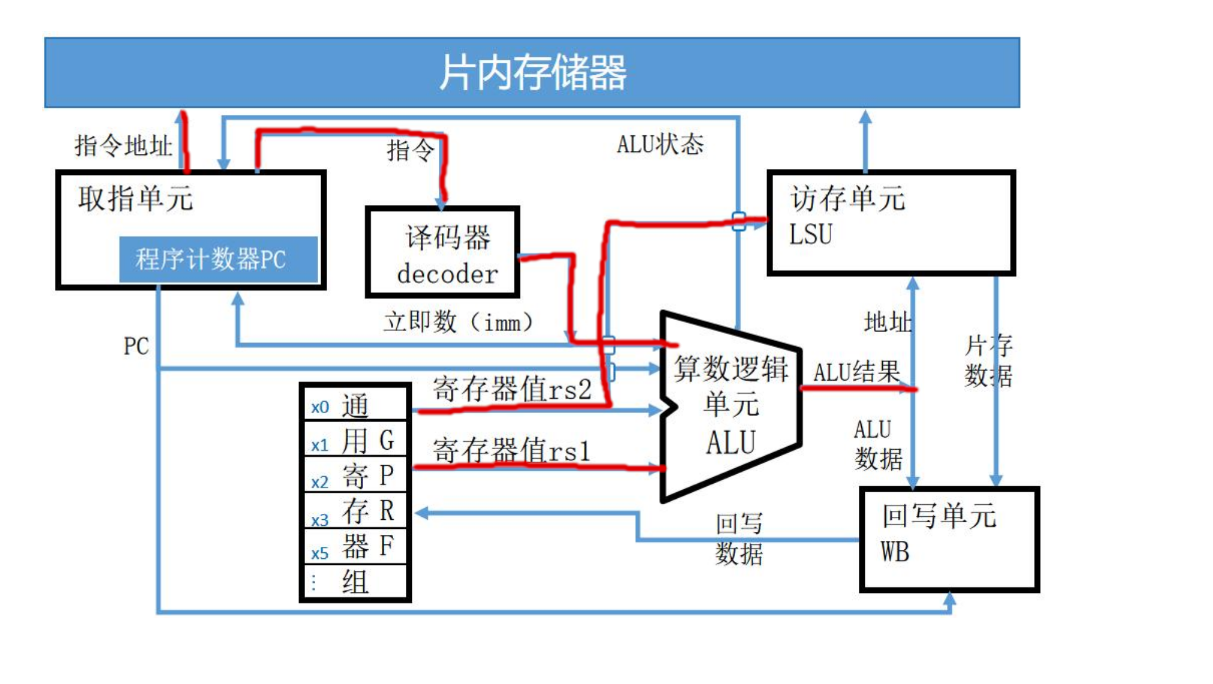
\includegraphics[width=0.8\textwidth]{sb.png} % 替换为图片路径
    \caption{sb数据通路}
    \label{fig:sb数据通路}
\end{figure}

\begin{verbatim}
      b4: fe744503     	lbu	a0, -0x19(s0)
      b8: fe042583     	lw	a1, -0x20(s0)
\end{verbatim}

为I型数据通路(读存储器),如下图所示
\begin{figure}[H]
    \centering
    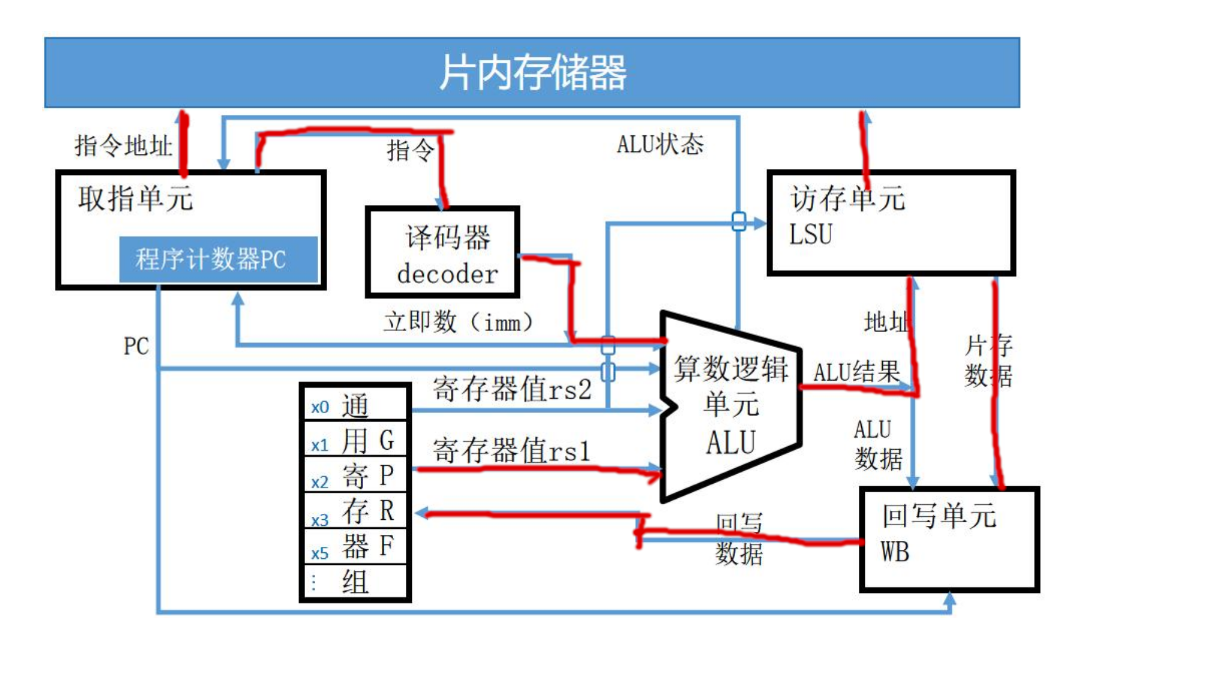
\includegraphics[width=0.8\textwidth]{I_read.png} % 替换为图片路径
    \caption{I型数据通路(读存储器)}
    \label{I型数据通路(读存储器)}
\end{figure}
\begin{verbatim}
bc: 00c585b3      add a1, a1, a2
\end{verbatim}

上述代码是I型数据通路(算术运算),如下图所示
\begin{figure}[H]
    \centering
    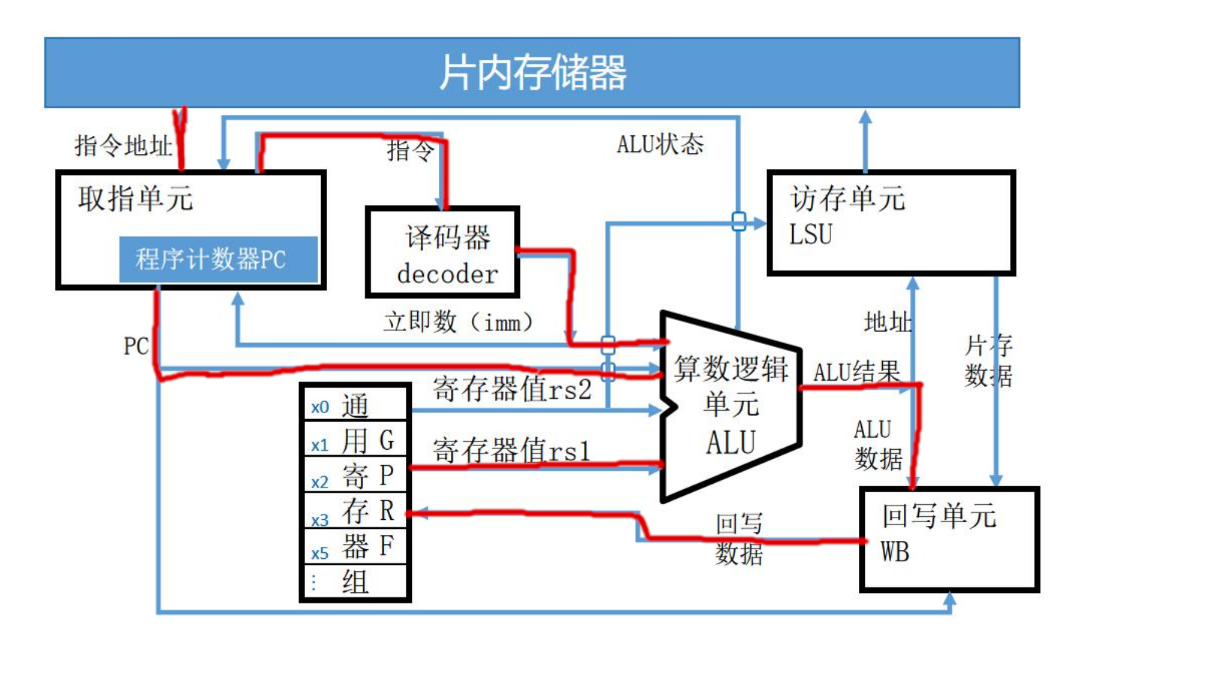
\includegraphics[width=0.8\textwidth]{I_cal.png} % 替换为图片路径
    \caption{I型数据通路(算术运算)}
    \label{I型数据通路(算术运算)}
\end{figure}
\begin{verbatim}
    c4: 0040006f     	j	0xc8 <.Ltmp5+0x78>
\end{verbatim}

是J型数据通路,如下图所示
\begin{figure}[H]
    \centering
    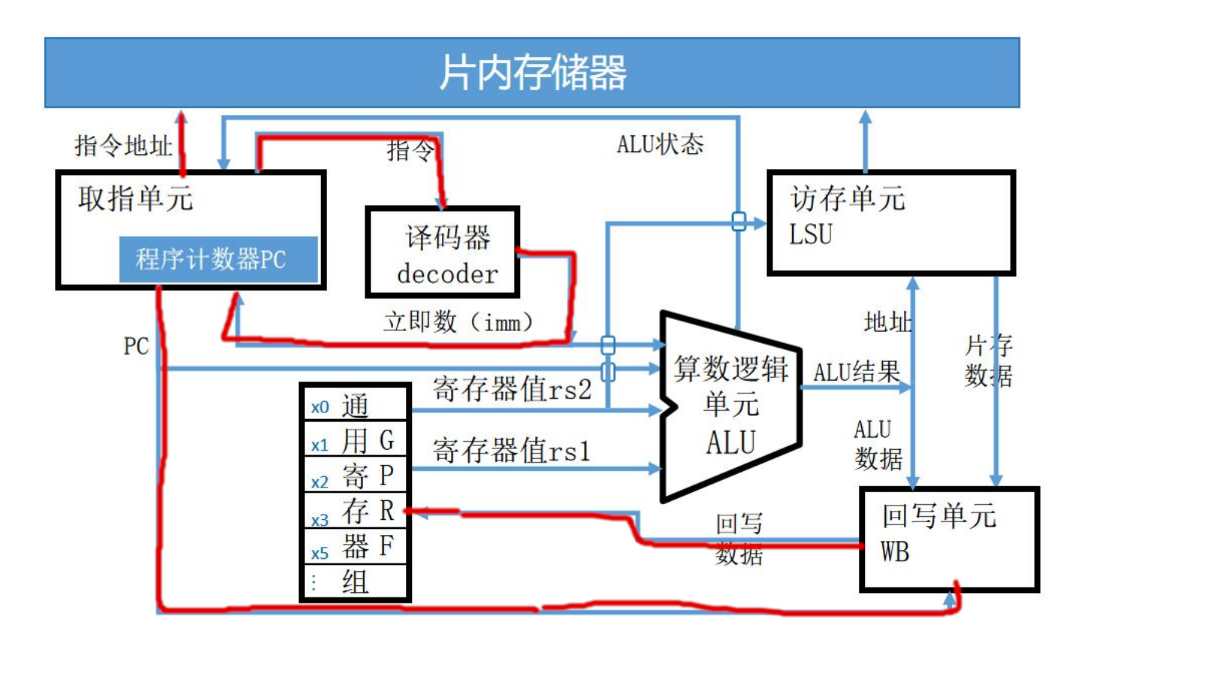
\includegraphics[width=0.8\textwidth]{J.png} % 替换为图片路径
    \caption{J型数据通路}
    \label{J型数据通路}
\end{figure}
\end{document}
